\documentclass[../main.tex]{subfiles}
\begin{document}
\setchapterstyle{kao}
\setchapterpreamble[u]{\margintoc}
\setchapterimage[6.5cm]{Images/eft.jpg}
\chapter[Effective Field Theories]{Effective Field Theories\footnotemark[0]}
\labch{EFT}
\section{Qualitative Introduction}
The \textbf{Standard Model} is a gauge theory based on SU$(3)\times$SU$(2)\times$U(1). There are no problems in extrapolating this theory at arbitrary high energies because there is the Higgs boson but like in QCD there is a problem on the quantum level due to U(1): the coupling explodes at extremely high energies ($\approx10^{42}$ GeV) hence it is an \textbf{effective field theory} (EFT).\marginnote{This is just a mathematical problem, before we can test this energy \textit{ne ha da passare di acqua sotto ai ponti}.} At the beginning of its formulation it was thought as a complete theory but now the modern viewpoint is that it is an EFT, there must be something else. This something else might appear at the Planck scale, where gravity also has to be realized in someway, or maybe it will appear much later, we do not know. By the way, the Standard Model also has other phenomenological problems: it does not account for dark matter, asymmetry between baryons and anti-baryons and other aspects which are not matching the experimental data. Everything which has to do with experiments in laboratory agrees perfectly with the Standard Model, but if we use it together with General Relativity to explain the Universe it fails badly. It does not include e.g. inflation, baryogenesis, dark matter and so on. In any case, the Standard Model needs to be expanded and now we have just discovered that because of its internal structure the theory is also mathematically incomplete.\\ 
We are forced to think a little bit about what are EFTs. Can we use them? These theories are not mathematically complete, but they are still important. Effective theories (\textit{not} effective field theories) are the way in which physics and science in general makes progress. This is called \textbf{reductionism}: we do not want to describe everything, we want to describe some set of phenomena in a certain domain of our parameters. For example, if we want to describe living bodies we do not need the know the fundamental constituents of matter. We can reduce the complexity of our problem providing an effective description. It is clear that we can always give an effective description as long as our system is described by at least two parameters which are vastly different and have the same dimensionality. 
\begin{example}
Classical mechanics is an effective theory of both quantum mechanics (for $l\gg h/p$) and special relativity (for $v\ll c$).
\end{example}
Our goal is to describe a relativistic QFT with very heavy degrees of freedom and study the behaviour at energies much lower than these degrees of freedom. Energy (or mass, equivalently) is our dimensionful quantity. It is possible to write an effective field theory where these degrees of freedom are not included, because there is not sufficient energy to create them but their effect can be captured in the effective theory by the addition of some local operators.\\
These theories are based on the concept of \textbf{locality}: the virtual exchange of heavy particles with mass $M$ happens at small distances, of the order of $1/M$. To give a qualitative explanation, we use the well known uncertainty principle, $\Delta E\Delta t\gtrsim\hbar/2$. There is an intrinsic limit for an instrument to measure both $E$ and $t$ simultaneously with a precision better than $\hbar/2$. Suppose to have an ideal instrument such that $\Delta E\Delta t\simeq\hbar/2$ and consider the virtual exchange of a heavy particle with mass $M$. We have a violation of momentum conservation since $M\gg p$ but this violation should not be observable because the particle gets emitted and lives for an extremely short time. 
\[
\Delta E\sim Mc^2\to\Delta t\sim\frac{\hbar}{2\Delta E}=\frac{\hbar}{2Mc^2}
\]
This is the precision on the time, which implies a precision on distance $\Delta x\simeq\frac{\hbar}{2Mc}$, therefore this propagation should take place at distances shorter than $\Delta x$ since this is the maximum we can measure. If instead we used a real instrument, we would obtain $\Delta x\approx\frac{\hbar c}{E}\gg \frac{\hbar}{2Mc}$: it is not possible to resolve the propagation of this heavy particle so the propagation of these particles will appear as a \textbf{local effect} in the theory.
\section{Structure of an Effective Lagrangian}
How can we describe local effects? With \textbf{local operators} which we have to include in our Lagrangian to take into account the contributions of these heavy particles. Our Lagrangian for an EFT will be:
\begin{equation}
\labeq{EFT}
\pazocal{L}_{\text{EFT}}=\pazocal{L}^{(4)}+\sum_n C^{(n)}O^{(n)}(x)
\end{equation}%1:19:37
$\pazocal{L}^{(4)}$ describes the low energy degrees of freedom and it is renormalizable while $O^{(n)}(x)$ are local operators of dimension $d_n$ which describe the effects of the heavy degrees of freedom. $C^{(n)}$ are arbitrary coefficients of dimension $4-d_n$ and they can be written in terms of a new scale, $C^{(n)}\propto\left(\frac{1}{M}\right)^{d_n-4}$, where $M$ denotes the mass of the heavy state. $\pazocal{L}_{\text{EFT}}$ is not renormalizable, however things are not so bad as they seem: let's have a look at the effects of these local operators. What does it mean \textit{local}? These are operators which are products, in general polynomial, of fields all computed in the \textbf{same point} with arbitrary dimensions. For example, $O(x)=\varphi^6(x)$ or $O(x)=(\Bar{\Psi}(x)\Psi(x))^2$. Then we add these operators according to the symmetries of our theory, they have to satisfy all the global symmetries that we impose on the low-energy theory.\marginnote{Gauge invariance is included among the symmetries.} There are two situations: \textit{either} we know the UV theory, find out what these operators are, take out the heavy particles and compare the two theories obtaining $C^{(n)}$ and then $O^{(n)}(x)$ \textit{or}, if we do not know the theory at high energy, write the most general effective Lagrangian compatible with symmetries we require at low-energy. Suppose to have an observable $A$ at low-energy, the relative effect of the heavy states, i.e. of the local operators, will be:
\[
\frac{\delta A}{A}\approx\left(\frac{E}{M}\right)^{(d_n-4)m}
\]
where $m$ is the number of insertions of the operator $O^{(n)}(x)$. The principal effects come from the low-energy degrees of freedom, there are corrections which go like $E/M$: the larger is the dimensionality of the operator, the smaller the effects will be. It is also possible to cut the series, since it does not have much sense to consider it all because of experimental precision we are not sensitive to these operators. The theory is not renormalizable, but we can truncate, so the number of parameters we have to renormalize is finite and we are happy. \raisebox{-\mydepth}{{
\includegraphics[height=1.1\baselineskip]{Images/smile.jpg}}}\\
When $M$ is much larger than the energy of the process we are considering it is possible to expand the propagator. But it is more convenient to expand the Lagrangian in terms of local operators which involve lighter degrees of freedom and the expansion is in terms of the ratio between the momenta of lighter particles and the mass $M$ of the heaviest particle, then truncate the series according to the precision required by the process.\\
To make things more clear, we make a couple of examples.
\subsection{Examples of EFTs}
\begin{example}\textbf{\href{https://en.wikipedia.org/wiki/Enrico_Fermi}{Fermi} theory for $\beta$ decay}\\
The $\beta$ decay $n\to pe^-\Bar{\nu}_e$ is described by:
\[
\pazocal{L}=-\frac{G_F}{\sqrt{2}}[\underbrace{\Bar{p}\gamma^\mu(1-\gamma_5)n}_{J^{\mu}_{\text{had}}}][\underbrace{\Bar{e^-}\gamma^\mu(1-\gamma_5)\nu_e}_{J^{\mu}_{\text{lep}}}]
\]
This Lagrangian is the product of two currents and has dimension 6. We can see it as an EFT obtained by integrating out, i.e. considering only what is below, a heavy particle coupled to both hadrons and leptons. This particle is massive with spin 1, with a mass much bigger than the energy involved in the process: the $W$ boson.\marginnote[-3cm]{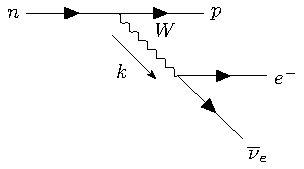
\includegraphics[]{Images/betadecay.pdf}\\
Diagram of the process}\\
From the complete theory, the amplitude of this diagram is given by:
\[
A=\left(\frac{g}{\sqrt{2}}\right)^2\frac{i^2}{2!}2\frac{(-i)}{k^2-m_W^2}\eta_{\mu\nu}\Bar{u}(p)\gamma^\mu\frac{(1-\gamma_5)}{2}u(n)\Bar{u}(e^-)\gamma^\nu\frac{(1-\gamma_5)}{2}v(\nu_e)
\]
Without going into details, the point here is that if $k^2\ll m_W^2$ it is possible to expand the propagator:
\[
\frac{1}{k^2-m_W^2}\simeq-\frac{1}{m_W^2}\left(1+\frac{k^2}{m_W^2}-\frac{k^4}{m_W^4}+\dots\right)
\]
Each term here is analytical in $k$, therefore each contribution comes from a local operator. The Fermi interaction is basically coming from the contribution at first order of this propagator, which means that the diagram is approximated by a contact interaction between the hadronic and leptonic currents. By comparing the amplitude from the effective theory with the one obtained by the complete theory (at first order) it is possible to find the value of the effective operator:
\[
\left(\frac{G_F}{\sqrt{2}}\right)=\frac{g^2}{8m_W^2}
\]
Higher order terms of the expansion correspond to other contributions, operators with higher dimensionality, where the momentum corresponds to derivative interactions acting on currents.
\[
\begin{aligned}
&\frac{k^2}{m_W^4}\to\frac{1}{m_W^4}J_{\text{had}}^\mu(x)\Box J_\mu^{\text{lep}}(x) \quad &&D=8\\
&\frac{k^4}{m_W^6}\to\frac{1}{m_W^6}J_{\text{had}}^\mu(x)\Box^2 J_\mu^{\text{lep}}(x) \quad &&D=10
\end{aligned}
\]
We are increasing the number of derivatives which act on the fields, hence the dimensionality. It is important that all these operators are local.
\end{example}
\begin{example}\textbf{Heavy fermion coupled to a scalar and a gauge field}\\
The Lagrangian which describes this kind of theory is:
\[
\pazocal{L}=\Bar{\Psi}(i\slashed{D}-M)\Psi-\frac{1}{4}(F_{\mu\nu})^2+\frac{1}{2}(\partial_\mu\phi)^2+y\phi\Bar{\Psi}\Psi-\frac{1}{2}m_\phi^2\phi^2
\marginnote[-2.5cm]{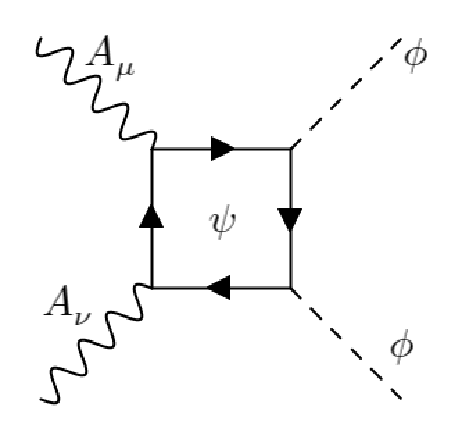
\includegraphics{Images/aaphiphi.pdf}\\
Diagram of the full process.}
\]
We want to take the limit in which $E\ll M$, where $\Psi$ will be point-like. It is possible to obtain an effective theory where $\Psi$ is not present but it is integrated out. What we get is a contact interaction between the scalar $\phi$ and the gauge field $A$ but since $\phi$ is neutral this interaction will not be of the type of minimal coupling but it will have to respect gauge invariance. \marginnote[-1cm]{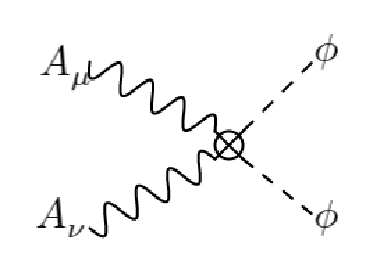
\includegraphics[0.5cm]{Images/phiplike.pdf}\\
Diagram for $E\ll M$ and $\Psi$ point-like.}
The operator involved will be $F^2_{\mu\nu}\phi^2$ which has dimension 6. The scattering amplitude will be:
\[
M(AA\to\phi\phi)\underset{\mathclap{\tikz \node {$\uparrow$} node [below=1ex] {\footnotesize $E\ll M$ };}}{\propto}\frac{g^2}{16\pi^2}y^2\varepsilon_\mu(p_1)\varepsilon_\nu(p_2)\underbrace{(\eta^{\mu\nu}(p_1\cdot p_2)-p_1^\mu p_2^\nu)}_{=M^{\mu\nu}}
\]
Gauge invariance, which implies the Ward identity, forces $M^{\mu\nu}$ to have this structure. The scattering amplitude has to be dimensionless, so there will be a mass scale at the denominator, given by $M^2$. The coefficient in front of the dimension 6 operator $F_{\mu\nu}^2\phi^2$ can be identified to be:
\[
c_6\simeq\frac{g^2}{16\pi^2}\frac{y^2}{M^2}
\]
Notice that the loop diagram is finite, because the superficial degree of divergence is zero. Gauge invariance forces us to have two powers of the external momenta and this lower the degree of divergence by two.
\end{example}
\section{EFTs as QFTs}
Let's get back to the general structure of an EFT [\refeq{EFT}]: what is the value of $d_n$? We have to be careful because in general the dimensionality of an operator can change with the interactions. If we assume that the EFT is weakly coupled, in a certain region of energy, then the dimensionality of $O^{(n)}(x)$ is the classical one. On the other hand, if the theory is strongly coupled, the dimensionality is modified by the interaction: there is an anomalous dimension coming from quantum effects. This anomalous dimension can be neglected in the case the theory is weakly coupled, so in our case $[O^{(n)}(x)]=d_n\simeq$ classical dimension.\\
The fact that for $E\ll M$ the contribution of high dimension operators is suppressed has some consequences: it implies that for $[O^{(n)}]>4$ they are irrelevant (in the IR), they become important at high energies. If we increase the energy, the contribution of these operators is increasing. At energy comparable to $M$, all the operators in the series will give contributions of the same order. At this point, the effective theory breaks down.\\
Suppose to have an EFT, where we have truncated the series and kept only the dominant contributions at low energy: how can we use this EFT? Can we use the Lagrangian only at tree-level or also at loop level? EFTs are \textbf{full-fledged QFTs}, there are no restrictions to impose, it is possible to use them at any loop order.\\
Take now a theory with quartic interaction and consider it at 1-loop. In this loop there is an exchange of virtual momenta which can be as large as we want. The derivatives appearing in the vertices will give us a nasty UV behaviour because the larger the number of derivatives is, the more divergent the diagram will be. The effective and the complete theory are different: in the complete theory, the loop has to be replaced with something with more propagators, which is more convergent. The UV behaviour is much nicer for complete theory than it is for effective ones but it is not a problem. These divergences will be local, they occur at very short distances since they correspond to extremely high virtual momenta so they basically correspond to local effect and they can be cancelled by the counter-terms. Being local operators, this is nothing but a redefinition of local operators that we insert in the theory. We are not changing the low energy behaviour. Let's see an example.
\begin{example}
Consider the following theory:
\[
\pazocal{L}=\frac{v^2}{4}\Tr{D_\mu\Sigma^\dagger D^\mu\Sigma} \quad \Sigma=\exp{i\frac{\chi^a(x)\sigma^a}{v}}
\]
If we expand in powers of $\chi$, we find:
\[
\pazocal{L}=(\partial_\mu\chi)^2+\frac{1}{v^2}(\chi\partial_\mu\chi)^2+\dots
\]
With other terms with increasing powers of the fields and therefore increasing dimensionality. From this expression, it is clear that there is a renormalizable part and one with higher dimension operators involving interaction. Suppose we want to expand it at 1-loop \marginnote[-1.5cm]{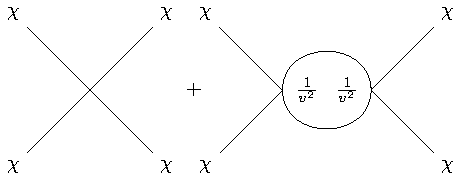
\includegraphics{Images/chiloop2.pdf}\\
1-loop expansion.}and for simplicity we consider $\chi$ massless. In each vertex, there are two derivatives and a factor $\frac{1}{v^2}$. We need to understand what is the factor compensating this $\frac{1}{v^4}$: we said that $\chi$ are massless so there will be nothing else but the external momentum.
\[
\text{loop contribution}\sim\frac{1}{v^4}\frac{1}{16\pi^2}p^4
\]
This will have a divergence of order $\log\left(-\frac{p^2}{\mu^2}\right)+\frac{1}{\varepsilon}$ where $\mu$ is the subtraction scale in dimensional regularization. To cancel this divergence, the counter-term has to be something like $(\partial_\mu\chi)^4$, with 4 derivatives and 4 fields. We have two possible local operators:
\[
(\Tr{\partial_\mu\Sigma^\dagger\partial_\nu\Sigma})^2 \quad (\Tr{\partial_\mu\Sigma^\dagger\partial^\mu\Sigma})^2
\]
This theory is not renormalizable but apart from the fact that we need increasing number of counter-terms is a standard QFT, so we can use this interaction without problems. 
\end{example}
If we work at low energy, it might be more convenient to use EFT than having the full theory because there will be less degrees of freedom. There are two possible EFTs:
\begin{enumerate}
    \item \underline{EFTs of known UV theories}: we use the so-called \textit{matching procedure}, i.e. choosing the effective coefficients so that the observables are equal in the EFT and in the complete UV theory. This is what we have done with the example of the Fermi theory.\\
    The UV theory does not have to be a field theory (e.g. it could be string theory) but we can still do matching. If the UV theory is instead a QFT we can do matching where the observable we compare are off-shell Green functions and we can impose a stronger constraint: the UV theory and the EFT reproduce the same Green functions.
    \item \underline{EFTs of unknown UV theories}: the coefficients are now unknown and there are 3 observations one can make.
    \begin{enumerate}
        \item EFT predicts quantities which are independent on the effective coefficients $C^{(n)}$, observables that are non-analytic in the momentum or in the parameters of the Lagrangian
        \item It is possible to extract the coefficients $C^{(n)}$ from experiments, or impose some limit on them
        \item We can make some estimates of $C^{(n)}$ and this requires power counting
    \end{enumerate}
\end{enumerate}
\begin{example}\textbf{QED as an EFT}\\
We want to consider the operator which contributes to the anomalous magnetic moment of the electron:
\[
c_0\underbrace{\Bar{\Psi}\sigma^{\mu\nu}F_{\mu\nu}\Psi}_{D=5}\quad\text{contributes to:}\left\{\begin{aligned}
&\Vec{\mu}=\frac{e}{2m_ec}g_e\Vec{s}\\
&a_e=\frac{g_e-2}{2}
\end{aligned}\right.
\]
where $\sigma^{\mu\nu}$ is a commutator between $\gamma$ matrices. If we go to low energies and compute the contribution of the vertex at tree-level, we get $\delta a_e^{\text{NP}}=\frac{4m_ec_0}{e}$. However, in QED we have also loop corrections, which give us $a_e\sim\frac{\alpha}{4\pi}$. Since QED is an EFT, we can imagine there are some heavy states that once integrated out will generate this local operator $c_0$ which gives the additional contribution. We want to make an estimate of $c_0$ in terms of parameters of the UV theory. We do not know exactly the details of this UV theory but it is possible to make some assumptions: there will be only one scale and one coupling strength to characterize this \textit{new} theory. At the end of the day, we then compare this result with the experimental one. This gives us:
\[
\frac{\delta a_e^{\text{exp}}}{a_e}=0.24\,\text{ppb}=2.4\cdot10^{-10}\marginnote{Best experimental result in physics, according to Contino.}
\]
We want to use this result to put some constraints on new physics and make predictions. In order to have complete predictions, we need to include also QCD. Considering now the 1-loop contribution coming from QCD, the precision of the theoretical prediction is:
\[
\frac{\delta a_e^{\text{th}}}{a_e}=6.7\,\text{ppb}=6.7\cdot10^{-9}
\]
About 30 times the experimental one! We can put some constraints on new physics by equating the contribution coming from $c_0$ with the largest theoretical uncertainty.
\[
\delta a_e^{\text{NP}}\lesssim\delta a_e^{\text{th}}\Rightarrow|c_0|\lesssim3\cdot10^{-9} \text{e/GeV}
\]
This is completely model independent, it does not make any assumption about what is the nature of this new physics contributing to this operator. If we want some more physical information about this new physics, we have to make assumptions and it is possible to make an estimation of the coefficient $c_0$ by using power counting:
\[
c^{(n)}\approx\left(\frac{1}{M_*}\right)^{d_n-4}g_*^{n-2}\left(\frac{g_*^2}{16\pi^2}\right)^l
\]
we denoted with $M_*$ the new physics scale, $n$ the number of fields in the operator $O^{(n)}$, $g_*$ the coupling strength in this new physics sector and $l$ the number of loops. $M_*$ is just the mass of the particle in the loop, assuming (1) there is just one particle and (2) there is only one coupling. These two assumptions are basically power counting. How do we apply all of this stuff in our case? Our operator has dimension $d_n=5$ and involves three fields $n=3$, so we get:
\[
c_0\sim\frac{e}{M_*}\left(\frac{g_*^2}{16\pi^2}\right)
\]
where we inserted the electromagnetic coupling $e$. The photon-electron interaction does not take place through the covariant derivative but via $F_{\mu\nu}$, it is a non minimal interaction. If the field of the new physics is minimally coupled with the covariant derivative there is no way to generate this operator at tree-level, we need one loop: that is another assumption we make (3). Suppose to have something like the diagram portrayed on the side: \marginnote[-3.5cm]{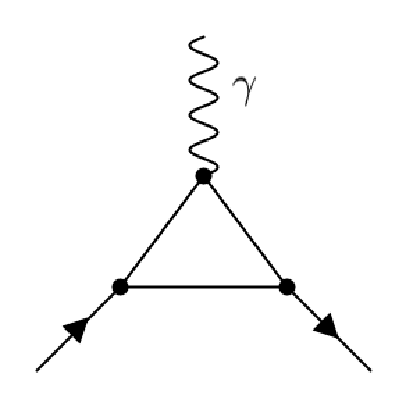
\includegraphics{Images/eftqed.pdf}}due to gauge invariance of electromagnetic theory, the coupling on the top vertex must necessary be $e$ while for the bottom vertex there is nothing that tells us it has to be some known coupling, so we denote the other coupling with $g_*$.\\
This is not the end of the story for our operator, there is still one extra-argument we can use. If we look at the structure of our operator, we notice that it is very similar to the structure of the mass term, mixing left and right chirality. There is a symmetry we can use: we know the mass term $\Bar{\Psi}_L\Psi_R$ is the only operator which breaks axial symmetry.
\[
P_A:
\left\{
\begin{aligned}
\Psi&\to\gamma^5\Psi\\
m_e&\to-m_e
\end{aligned}
\right.
\]
$m_e(\Bar{\Psi}_L\Psi_R+\text{h.c.})$ is formally invariant under $P_A$. Another assumption (4) is that there is only one spurion in the new theory which breaks $P_A$ and it is the same which contributes to the mass term and to the new operator. This implies that this operator must be proportional to $m_e$:
\[
c_0\sim\frac{e}{M_*}\left(\frac{g_*^2}{16\pi^2}\right)\frac{m_e}{M_*}
\]
So it is not dimension 5 but dimension 6, giving an additional suppression. The interesting quantities characterizing the new physics are $M_*$ and $g_*$, we can establish a constraint for $M_*$:
\[
M_*\gtrsim3\,\text{GeV}\cdot g_*
\]
The coupling cannot be larger than $4\pi$ or it would not be perturbative anymore. This tells us that the correction to new physics will be under experimental precision if $M_*$ is larger than the value we just found.\\
This new physics is just the Standard Model completion of QED+QCD and the particles contributing in the loops are the vector bosons.
\[
\left\{
\begin{aligned}
&m_W\simeq80\,\text{GeV}\\
&m_Z\simeq90\,\text{GeV}\\
&m_h\simeq125\,\text{GeV}
\end{aligned}
\right.
\to
\left\{
\begin{aligned}
&M_*\approx100\,\text{GeV}\\
&g_*\sim g\sim0.65
\end{aligned}
\right.
\]
The anomalous magnetic moment of the electron is not sensitive to new physics of this kind, because its scale is too heavy. However, there is another situation where we are sensitive to new physics because $c_0$ scales with $m_e$ so at this point we ask ourselves if we can consider the muon magnetic moment instead of the electron one. The experimental precision for the muon anomalous magnetic moment is\\
0.35 ppm $=3.5\cdot10^{-7}$ and with this result we get $M_*\approx400\,\text{GeV}\cdot g_*$, the same order of magnitude as before. In the Standard Model, the operator is modified:
\[
c_0\Bar{\Psi}\sigma^{\mu\nu}F_{\mu\nu}\Psi\to\Bar{\Psi}_L\sigma^{\mu\nu}W^{\mu\nu}\Psi_RH\marginnote{At the moment this formula is a bit beyonf our understanding, but it will become more clear (hopefully) after the next chapter.}
\]
$H$ is the Higgs field, required to have SU$(2)_{\text{EW}}$ invariance. Now we have $\Delta a_\mu=a_\mu^{\text{exp}}-a_\mu^{\text{SM}}=2.5\cdot10^{-9}$ which is larger than experimental uncertainty. There is a difference at $4\sigma$ level, so there must be some new physics. We can say that this difference comes from $W^{\mu\nu}$ and if we do this we get a scale
$M_*\approx25\,\text{GeV}\cdot g_*$. This is a bit uncomfortable because it is below the electroweak scale, the new physics should be lighter than the electroweak particles \textit{unless} the coupling gets larger.
\end{example}
\section{Validity of EFTs}
When these effective theories collapse? There is not a unique answer, we have to make some assumptions (again). Let's see an example.
\begin{example}\textbf{Fermi theory}\\
\[
\pazocal{L}=c_6[\Bar{e}\gamma^\mu(1-\gamma^5)\nu_e][\Bar{\nu}_\mu\gamma_\mu(1-\gamma^5)\mu] \quad c_6=-\frac{G_F}{\sqrt{2}}=-\frac{g^2}{8m_W^2}\marginnote[-1cm]{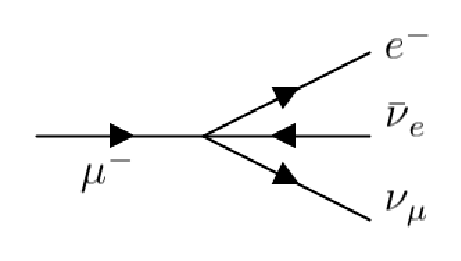
\includegraphics[]{Images/fermieft.pdf}}
\]    
This operator describes the purely leptonic decay of the muon depicted on the side. If we compare it with the effective operator for protons, neutrons, electrons and neutrinos the coefficient in front is not quite the same but approximately the same. Suppose to measure the muon lifetime, what is measured is the coefficient $c_6$. Since in our theory there is nothing to justify the decay of the muon, then we understand that this process is mediated by effective operators, hence why we want to measure $c_6$. What does this say about the scale of new physics? It does not tell us anything directly about the scale of new physics because what we measure is the ratio between the coupling and the scale: without knowing the value of the coupling we cannot say anything about the scale. Today, we know the value of the coupling since the full theory is known but at the time when people first observed the muon decay this information was not available. What is the range of possibility? We can vary the coupling from very small values up to 4$\pi$, where the theory becomes not perturbative. \marginnote{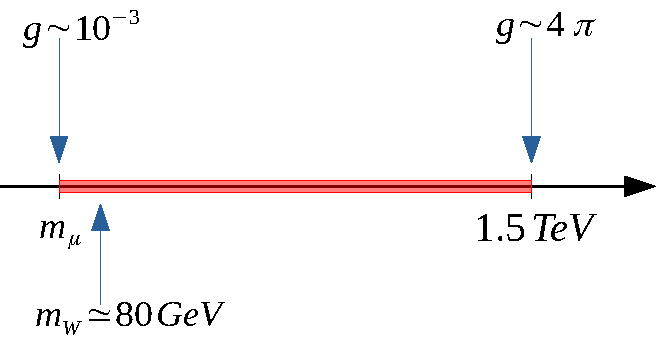
\includegraphics[-1cm]{Images/scalenp.pdf}} The scale of new physics varies between the mass of the muon up to a point where the coupling is of order 4$\pi$, corresponding to the scale of new physics of order 1.5 TeV. This range is highlighted in red in the picture on the side, but we do not know exactly where this new physics could appear. How could we determine it? We \textit{either} make some assumptions on the value of the coupling, which of course have to be theoretically motivated, and then extrapolate the value of $m_W$ \textit{or} we look for new physics in scattering processes with the same elements of the Fermi interaction, for example $e^-\nu_\mu\to\mu^-\nu_e$. This was done by the Gargamella experiment in 1973, observing both charged and neutral currents, so $W$ and $Z$. To find the masses, we had to wait until 1983 at CERN which told us that this new physics appears at $m_W\simeq80$\,GeV.
\end{example} 
\end{document}
%QFT beyond tree-level (QED a 1 -loop con Barducci)
%Symmetries and conservation laws (spontaneous symmetry breaking and Higgs mechanism)
%Quick intro to non-abelian gauge theories
%Effective field theories
%Intro to the SM